\documentclass[graybox]{svmult}

\usepackage{type1cm}
\usepackage{makeidx}         
\usepackage{multicol}        
\usepackage[bottom]{footmisc}
\usepackage{newtxtext}  
\usepackage{newtxmath}  
\usepackage[dvipdfmx]{graphicx}
%\usepackage{graphicx}	
\usepackage{bm}
\usepackage{url}

\usepackage{listings}
\lstset{
frame=trbl,
numbers=left,
numbersep = 7pt,
tabsize=1,
columns=[l]{fullflexible},
language = C
}

\usepackage{algorithmic,algorithm}

\begin{document}

\title*{
  XcalableMP 2.0 and Future Directions
}

\titlerunning{
  XcalableMP 2.0 and Future Directions
}

\author{Mitsuhisa Sato, Hitoshi Murai, Masahiro Nakao, Keisuke Tsugane, Tesuya Odajima
  and Jinpil Lee}

\institute{
  Mitsuhisa Sato \at RIKEN Center for Computational Science, Kobe, JAPAN
  \email{msato@riken.jp}
\and 
  Hitoshi Murai \at RIKEN Center for Computational Science, Kobe, JAPAN
  \email{h-murai@riken.jp}
\and 
  Masahiro Nakao \at RIKEN Center for Computational Science, Kobe, JAPAN
  \email{masahiro.nakao@riken.jp}
\and 
Keisuke Tsugane\at Fujitsu Laboratories Ltd., 4-1-1 Kamikodanaka,
Nakahara-ku, Kawasaki, Kanagawa 211-8588, JAPAN
\email{tsugane.keisuke@fujitsu.com}
\and
  Tetsuya Odajima \at RIKEN Center for Computational Science, Kobe, JAPAN
  \email{tetsuya.odajima@riken.jp}
\and 
  Jinpil Lee \at RIKEN Center for Computational Science, Kobe, JAPAN
  \email{jinpil.lee@riken.jp}
}

\maketitle

\abstract*{
  This chapter presents the XcalableMP on the Fugaku supercomputer,
  the Japanese flagship supercomputer developed by FLAGSHIP2020 project in RIKEN R-CCS. The porting and the performance evaluation are done as a part of this project, and the XcalableMP will be available for the Fugaku users for improving the productivity and performance of parallel programing.
  The performance of XcalableMP on the Fugaku is enhanced by the manycore processor and a new Tofu-D interconnect.  
  We are now working on the next version, XcalableMP 2.0, for cutting-edge high-performance systems with manycore processors by multithreading and multitasking with integrations of PGAS model and synchronization models.
 We conclude this book with retrospectives and challenges for future PGAS models.
}

\abstract{
  This chapter presents the XcalableMP on the Fugaku supercomputer,
  the Japanese flagship supercomputer developed by FLAGSHIP2020 project in RIKEN R-CCS. The porting and the performance evaluation are done as a part of this project, and the XcalableMP will be available for the Fugaku users for improving the productivity and performance of parallel programing.
  The performance of XcalableMP on the Fugaku is enhanced by the manycore processor and a new Tofu-D interconnect.  
  We are now working on the next version, XcalableMP 2.0, for cutting-edge high-performance systems with manycore processors by multithreading and multitasking with integrations of PGAS model and synchronization models.
 We conclude this book with retrospectives and challenges for future PGAS models.
}

\section{Introduction}

We have been developing a production-level XcalableMP compiler, and make it available for the K computer’s users as well as the users of conventional clusters.
RIKEN R-CCS has been carrying out the FLAGSHIP 2020 Project\cite{FLAGSHIP2020} to develop the Japanese flagship supercomputer system following the K computer,
the Post-K, formally named as "Fugaku" later, since 2014. 
In the project, 
XcalableMP was taken as a parallel programming language project
for improving the productivity and performance of parallel programing.
XcalableMP is now available on Fugaku and the performance is enhanced by the Fugaku interconnect, Tofu-D. The next section describes the XcalableMP on Fugaku.

The XcalableMP project has been started from 2008 and the discussion on XcalableMP 1.x has converged. We are now working on a new version, XcalableMP 2.0, targeted for cutting-edge high-performance systems with manycore processors by multithreading and multitasking with integrations of PGAS model and synchronization models.
In this new programming model, the execution of the program is decomposed into several tasks executed according the dependency between tasks. This model will enable less overhead of synchronization eliminating expensive global synchronization, overlap between computation and communication in manycore, and light-weight communication by RDMA in PGAS model.
We will extend this programming model to combine several kinds of accelerators such as GPU, FPGA and special-purpose processors with large-scale general-purpose manycore systems. It enables some task to be offloaded into the accelerators such as FPGA as well as each core in modern manycore processor. We consider this configuration as a general global architecture of the future system as some part of system will be specialized for high performance and power efficiency. Our programming model will make it easy to adopt the existing computational science program to the new systems.

In Section 2, a proposal for XcalableMP 2.0 is presented,
followed by retrospectives and challenges for future PGAS models in Section 3.

\section{XcalableMP on Fugaku}

In this section, we report our early experience and the preliminary performance of XcalableMP on Fugaku.
The Fugaku is a huge-scale system with general-purpose manycore processors.
The node processor is a single chip, named Fujitsu A64FX, which consists of 48 cores with 2 or 4 cores dedicated for OS activities, 32 GiB HBM2 memory, with TofuD interconnect, and a PCI express controller in the chip together.
The Fugaku system consists of 158,976 nodes in 432 racks.
The Fugaku is scheduled to be put into operation for public service around 2021. In 2020, the installation is completed and the system partially serves the early-access program. 

XcalableMP is available as a parallel programming language for the Fugaku, supported by R-CCS team with Fujitsu. C and Fortran are supported as base languages with XcalableMP 1.2 compliant.

We report the preliminary performance of XcalableMP program running on the Fugaku
\footnote{
The reported results were obtained on the evaluation environment in the trial phase.
Note that the performance is not guaranteed at the start of its operation.}.

We used the following versions:
\begin{itemize}
\item Omni XcalableMP Version: 1.3.2, Git Hash:6d23f46
\item Language specification: 1.2.25
\end{itemize}

The performance of XcalableMP on the Fugaku is enhanced by the manycore processor and a new Tofu-D interconnect.  

\subsection{Performance of XcalableMP Global View Programming}

We executed the IMPACT-3D, described in Chapter 6, for the evaluation of XcalableMP global view programming in the Fugaku, using up to 512 nodes.
The scalability on Fugaku is shown in Figure \ref{fig-impact3D},
comparing to the K computer. The program is parallelized by hybrid XMP-OpenMP parallel programming: An XMP node is assigned to a node, and 48 OpenMP threads are running within a node. The problem size is $512 \times 512 \times 512$ with 3-dimensional block distribution. The compile option is ``-Kfast''.

As shown in the figure, we found a good scalability in Fugaku, and the performance is better than that by MPI thanks to the optimized XMP runtime for communications in the stencil computation\cite{Murai2013}.

\begin{figure}[thb]
\begin{center}
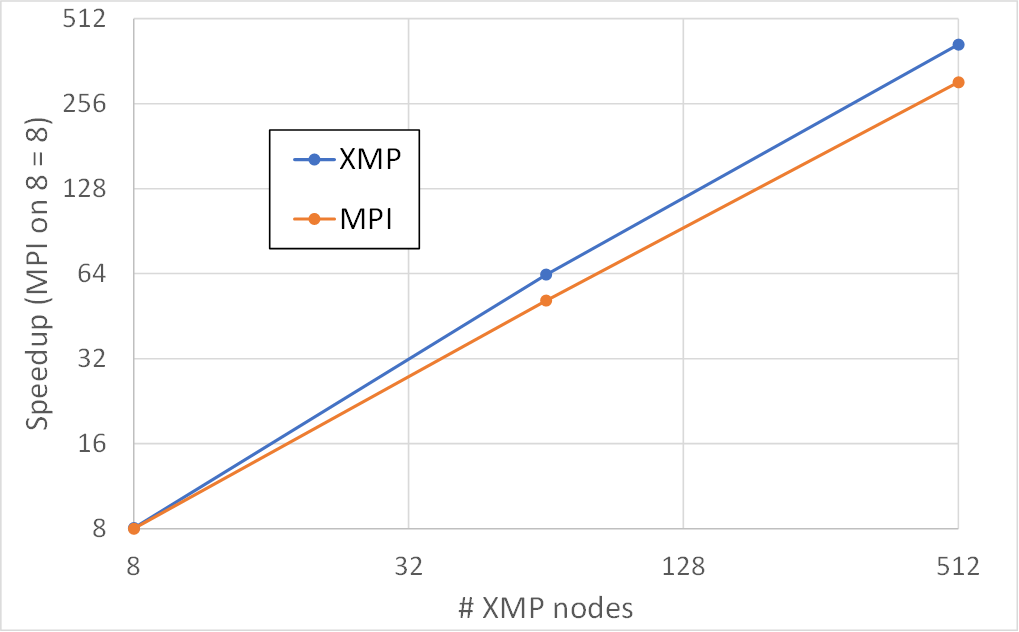
\includegraphics[width=8cm]{./figure/Perf-impact3D.png}
\caption{Speedup of Impact3D on Fugaku and Performance comparing to K computer}
\label{fig-impact3D}
\end{center}
\end{figure}

\subsection{Performance of XcalableMP Local View Programming}

Fugaku has a customized interconnection, called Tofu-D, which supports hardware-supported RDMA (Remote Direct Memory Access) operations. We implemented the XMP runtime library to make use of Tofu-D for one-sided communication for the XMP local view programming. The library is implemented by using a low-level communication layer, uTofu API \cite{uTofu}, provided by Fujitsu.

For performance evaluation of XMP local view programming,
we used CCS QCD and NTChem-MINI taken from the coarray version of Fiber Miniapp Suite \cite{Fiber}\cite{Murai2017}.

To run CCS QCD mini-application\cite{CCS-QCD}, 8 XMP nodes are assigned to one node, running in a flat XMP mode.
The size and conditions are as follows:

\begin{itemize}
\item Target data: Class 2 (32 x 32 x 32 x 32) (strong scaling)
\item Compiler options: -Kfast,zfill,simd=2
\item Timing region: sum of ``Clover + Clover\_inv Performance''
and ``BiCGStab(CPU:double precision) Performance''” of the
built-in timing feature
\end{itemize}

Figure \ref{fig-QCD} shows the speedup of the Fugaku,
comparing to the performance of the K computer.
The XMP version archives almost same performance of the MPI version.
Note that the reason of the performance degradation of the XMP version on the K computer is the overhead of allocation for allocatable coarray used as a buffer for communication. It is improved by removing this overhead by using the uTofu communication layer.

\begin{figure}[thb]
\begin{center}
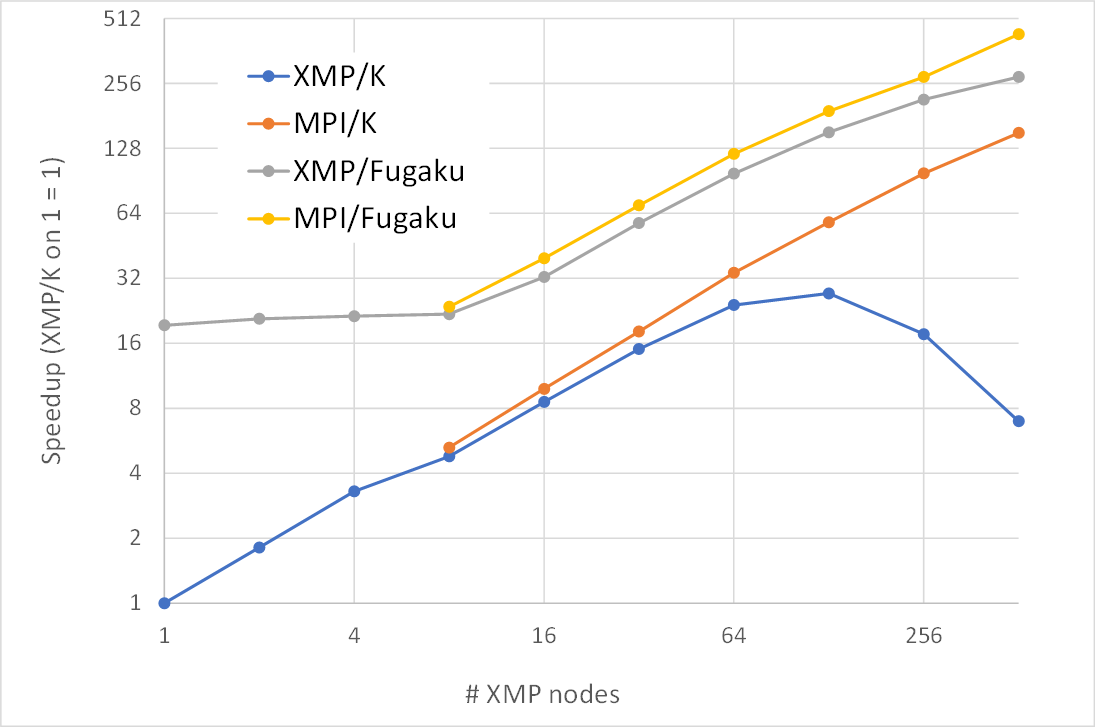
\includegraphics[width=8cm]{./figure/Perf-QCD.png}
\caption{Speedup of CCS QCD on Fugaku and Performance comparing to the K computer}
\label{fig-QCD}
\end{center}
\end{figure}

The NTChem-MINI is a mini-application taken from NTChem \cite{NTChem}, a high-performance software package for molecular electronic structure calculation. An XMP node is assigned to one node, and within a node, BLAS functions are executed using 48 cores.
The size and conditions are set as follows:

\begin{itemize}
\item Target data: taxol (strong scaling)
\item Compiler options: -Kfast,simd=2
\item Timing region: “RIMP2\_Driver” of the built-in timing feature
\end{itemize}

As shown in Figure \ref{fig-NTchem}, the XMP versions archive almost the same performance of the original MPI versions.

\begin{figure}[thb]
\begin{center}
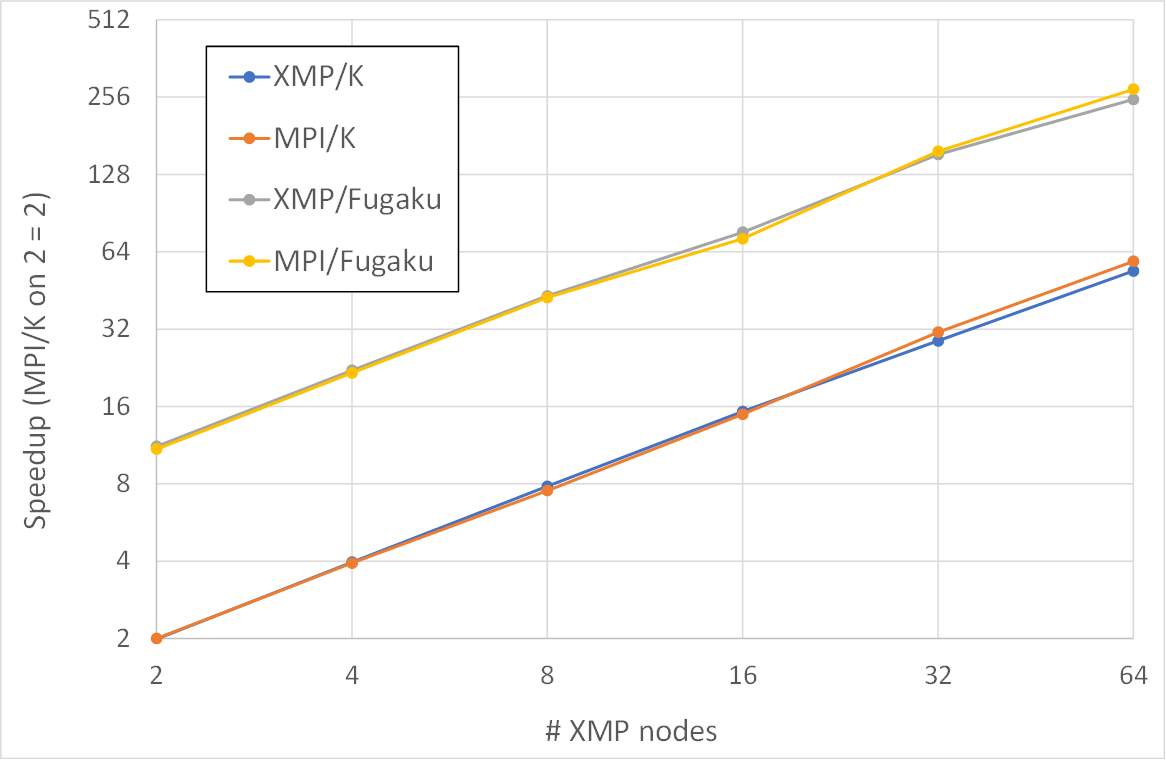
\includegraphics[width=8cm]{./figure/Perf-NTchem.png}
\caption{Speedup of NTChem-MINI on Fugaku and Performance comparing to the K computer}
\label{fig-NTchem}
\end{center}
\end{figure}

\section{Global Task Parallel Programming}

Recently, large-scale clusters of many-core processor such as Intel Xeon Phi have been deployed in many sites from the latest Top500 Lists. In order to program many-core processors, OpenMP is widely used as a shared-memory programming model. Most of OpenMP programs are written using work sharing constructs for loops, which involves a global synchronization.
However, especially in modern many-core processors, the global synchronization cost for work sharing becomes bigger, and the load imbalance among cores lead to the performance degradation as the number of cores on the processor increases.
Task parallel programming using task dependency in OpenMP 4.0 is a promising candidate to facilitate the parallelization for such many-core processors because it enables users to avoid global synchronization by fine-grained task-to-task synchronization through user-specified data dependencies.

We are interested in extending the task parallel programming model to the PGAS model of XcalableMP for distributed memory systems.
As well as removing expensive global synchronization,
it is expected to enable the overlapping of communication and computation.
In XMP 2.0, we propose the global task parallel programming.

In OpenMP, the task dependency in a node depends on the order of reading and writing to data based on the sequential execution. Therefore, the OpenMP multi-tasking model cannot be applied to describe the dependency between tasks running in different nodes since threads of each nodes are running in parallel. In OmpSs, interactions between nodes are described through the MPI task that is executing MPI communications. Task dependency between nodes is guaranteed by the completion of MPI point-to-point communication in tasks. 

We propose new directives for communication with tasks in XMP, and they enable users to write easily the multi-tasking execution based on XMP language constructs. The tasklet directive generates a task for the associated structured block
 on the node specified by the on clause, and the task is scheduled and immediately executed by an arbitrary thread in the specified node if there is no task dependency. If it has any task dependencies, the task execution is postponed until all dependencies are resolved. The tasklet gmove directive copies the variable of the right-hand side (rhs) into the left-hand side (lhs) of the associated assignment statement for local or distributed data in tasks. If the variable of the rhs or the lhs is the remote data, this directive may synchronize on data dependency between nodes and execute communication. The tasklet reflect directive is a task-version of reflect operation. It updates halo regions of the array specified to array-name in tasks. In this directive, data dependency is automatically added to these tasks based on the communication data because the boundary index of the distributed data is dynamically determined by XMP runtime system.

We have designed a simple code translation algorithm from the proposed directives to XMP runtime calls with MPI and OpenMP. We have evaluated the performance using block-Cholesky Factorization Program on KNL based-system, Oakforest-PACS. Through the experiment, we confirmed the advantage of task-parallelism over the traditional loop-based data parallelism. At the same time, we found the performance problems on communication between multiple threads (MPI\_THREAD\_MULTIPLE). Currently, we are investigating a lower-level communication API for efficient one-sided communication of PGAS operations in multithreaded execution environment.

Details of the proposal in this chpater are decribed in \cite{HPCAsia2018}.

\subsection{OpenMP and XMP Tasklet Directive}

While OpenMP originally focuses on work sharing for loops as the {\tt parallel for} directive, OpenMP 3.0 introduces task parallelism using the {\tt task} directive. It facilitates the parallelization where work is generated dynamically and irregularly as in recursive structures or unbounded loops. The {\tt depend} clause on the {\tt task} directive is supported from OpenMP 4.0 and specifies data dependencies with dependence-type {\tt in}, {\tt out}, and {\tt inout}. Task dependency can reduce the global synchronization of a thread team because it can execute fine-grained synchronization between tasks through user-specified data dependencies.

To support task parallelism in XMP as in OpenMP, the {\tt tasklet} directive\footnote{There is the {\tt task} directive in XMP, it is different from OpenMP’s one.} is proposed in XMP 2.0. Fig. \ref{FIG_TASKLET} describes the syntax of the {\tt tasklet}, {\tt tasklets}, and {\tt taskletwait} directives for the multi-tasking execution in XMP. The {\tt tasklet} directive generates a task for the associated structured block on the node specified by the {\tt on} clause, and the task is scheduled and immediately executed by an arbitrary thread in the specified node if there is no task dependency. If it has any task dependencies, the task execution is postponed until all dependencies are resolved. These behaviors occur when these tasks are surrounded by {\tt tasklets} directive. When these tasks are not surrounded by the {\tt tasklets} directives, they are executed sequentially at the specified node. The {\tt tasklet} directive supports several clauses for the description of the task dependency. The {\tt in}, {\tt out}, and {\tt inout} clauses represent the task dependency in a node. When {\tt in}, {\tt out}, or {\tt inout} clause presents on the {\tt tasklet} directive, the generated task has each data dependency in a node. The behavior of these data dependencies is same as OpenMP {\tt task depend} clause: flow, anti, and output dependencies. 

The {\tt taskletwait} directive waits on the completion of the generated tasks on each node. Since the directive does not involve the barrier synchronization, the {\tt barrier} directive in XMP is also required in order to guarantee that all tasks of all nodes are finished at this point. There is an implicit barrier on each node at the end of the {\tt tasklets} directive.

In OpenMP, the task dependencies are created according to the order of reading and writing to data based on the sequential execution in a node.
Therefore, the OpenMP task parallel model cannot be directly applied to describe the dependency between tasks running in different nodes since threads of each nodes are running in parallel.

In OmpSs\cite{OMPSS}, interactions between nodes are described through the MPI task that is executing MPI communications. Task dependency between nodes is guaranteed by the completion of MPI point-to-point communication in tasks. While this approach can satisfy dependencies between nodes, it may cause further productivity degradation because it forces users to use a combination of two programming models that are based on different description formats. Therefore, we propose new directives for communication with tasks in XMP, and they enable users to write easily the multi-tasking execution for clusters by only using language constructs.

\begin{figure}[t]
\begin{center}
\setbox0\vbox{\scriptsize
\hbox{{\bf \#pragma} {\tt xmp tasklet} {\it [clause[, clause] ... ]} {\it [on \{ node-ref $|$ template-ref \} ] }}
\hbox{\quad (structured-block)}
\hbox{}
\hbox{{\bf \#pragma} {\tt xmp taskletwait} {\it [on \{ node-ref $|$ template-ref \} ] }}
\hbox{}
\hbox{{\bf \#pragma} {\tt xmp tasklets}}
\hbox{\quad (structured-block)}
\hbox{}
\hbox{\quad where {\it clause} is :}
\hbox{\qquad \{{\tt in} $|$ {\tt out} $|$ {\tt inout}\} ({\it variable[, variable] ... ]})}
}
\centerline{\fbox{\box0}}
  \caption{Syntax of the {\tt tasklet}, {\tt taskletwait}, and {\tt tasklets} directives in XMP.}
  \label{FIG_TASKLET}
\end{center}
\end{figure}

\subsection{A Proposal for Global Task Parallel Programming}

In order to achieve multi-tasking execution for distributed memory parallel systems, we need to perform point-to-point communication within tasks in local task dependency graphs. While XMP provides some directives for communication, many of these are performed collectively, and cause an implicit synchronization among execution nodes. This causes a performance degradation, because tasks participating in communications, such as broadcast, wait for synchronization until all tasks are completed. In this paper, we propose two directives, {\tt tasklet gmove} and {\tt tasklet reflect}, as shown in Fig. \ref{FIG_TASKLET_COMM}, to describe interactions between nodes in tasks by point-to-point communication, for inter-node data dependency. These communications are only synchronized between the sender and receiver of the communication in each task. 

These details are as follow:

{\tt tasklet gmove} directive: Although this copies the variable from the right-hand side (rhs) into the left-hand side (lhs) of the associated assignment statement for local or distributed data like the {\tt gmove} directive, it is executed in tasks. The copy operation is basically performed on all execution nodes. However, if the distributed array is specified at the associated assignment statement, only nodes with the distributed array execute the operation in the task. The execution nodes can also be determined by the {\tt on} clause. When the {\tt in}, {\tt out}, or {\tt inout} clause is present on the {\tt tasklet gmove} directive, the generated task has the corresponding data dependency in a node, similar to the {\tt tasklet} directive. While the {\tt gmove} directive also supports one-sided communication by the {\tt in} and {\tt out} clauses, which differ from those used for data dependencies, the {\tt tasklet gmove} directive does not support these in this work.

{\tt tasklet reflect} directive: Although this update halo regions of the array specified to {\tt array-name} like the {\tt reflect} directive, it is executed in tasks. For example, when updating one side of a halo region for a one-dimensional distributed array on two nodes, these communications are separated into four tasks: the sender of the upper element on node 1, the receiver of the upper halo region on node 1, the sender of the lower element on node 2, and the receiver of the lower halo region on node 2. In this directive, data dependency is automatically added to these generated tasks based on the communication data, because the boundary index of the distributed array is dynamically determined by the XMP runtime system. The {\tt chunksize} clause can be matched the task dependency descriptions of users using the dependency generated by the {\tt tasklet reflect} directive. When users calculate an array in block units, such as in the cache blocking technique for a node with data dependency, the user-specified task dependency and generated data dependency for halo exchange may not identically match. By specifying the {\tt chunksize} clause, the halo region is distributed logically to equal-sized contiguous chunks, and data dependencies for the halo exchange are generated automatically by the XMP runtime system based on the specified chunk size. 

Fig. \ref{FIG_TASKLET_GMOVE} presents an example of the {\tt tasklet gmove} directive. In this example, array {\it A[]} with length three is distributed to three nodes in equal-sized contiguous blocks. This code creates three kinds of tasks. TaskA and taskC are executed on nodes specified by the {\tt on} clause. TaskB is executed on nodes 1 and 2, because these nodes have the specified distributed array {\it A[0]} or {\it A[1]} in the associated assignment statement under the {\tt tasklet gmove} directive. There is a flow dependency between taskA and taskB on node 1 by {\it A[0]}. After the execution of taskA, taskB sends {\it A[0]} to node 2, which is determined by the distributed array {\it A[1]}. In node 2, taskB receives {\it A[0]} from node 1 in {\it A[1]}. When the receive operation in taskB is finished, taskC is immediately started, because the flow dependency of {\it A[1]} is satisfied. TaskC sends the {\it A[1]} to variable {\it B} of node 3. Because the variable {\it B} is a local variable for each node, the communication destination is determined from the execution nodes specified by the {\tt on} clause.

\begin{figure}[t]
\setbox0\vbox{\scriptsize
\hbox{{\bf \#pragma} {\tt xmp tasklet gmove} {\it [clause[, clause] ... ]} {\it [on \{ node-ref $|$ template-ref \} ] }}
\hbox{\quad (an assignment statement)}
\hbox{}
\hbox{{\bf \#pragma} {\tt xmp tasklet reflect} {\it (array-name[, array-name] ... )}}
\hbox{\qquad\qquad\qquad\qquad\qquad {\it [blocksize (reflect-blocksize[, reflect-blocksize] ... ) ]}}
\hbox{}
\hbox{\quad where {\it clause} is :}
\hbox{\qquad \{{\tt in} $|$ {\tt out} $|$ {\tt inout}\} ({\it variable[, variable] ... ]})}
}
\centerline{\fbox{\box0}}
\caption{Syntax of the {\tt tasklet gmove} and {\tt tasklet reflect} directives in XMP}
\label{FIG_TASKLET_COMM}
\end{figure}

\begin{figure}[t]
\begin{center}
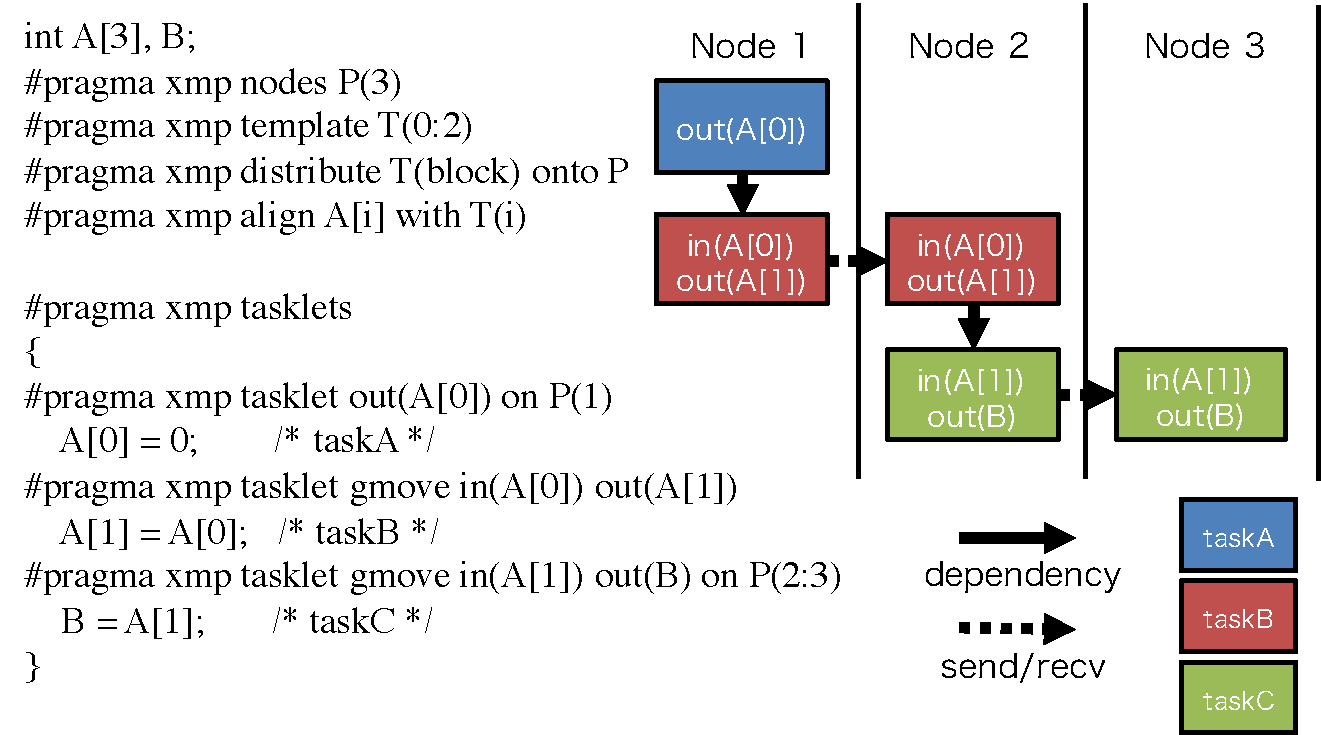
\includegraphics[bb=0 0 509 385, width=6.7cm]{./figure/FIG_TASKLET_GMOVE.pdf}
\caption{Example of the {\tt tasklet} and {\tt tasklet gmove} directives.}
\label{FIG_TASKLET_GMOVE}
\end{center}
\end{figure}


\subsection{Prototype Design of Code Transformation} \label{SEC_CODE_TRANSLATION}

We have designed a simple code transformation from the code using the proposed directives to the code with XMP runtime calls using MPI and OpenMP. 
As for a preliminary evaluation, we have made a hand-translated MPI and OpenMP code by using the proposed transformation.

The {\tt tasklets} directive is converted into the OpenMP {\tt parallel} and {\tt single} directives. The execution node is determined by the {\tt on} clause, which is translated to an {\tt if} statement. The {\tt tasklet gmove} and {\tt tasklet reflect} directives are converted into MPI\_Send/Recv(), and these MPI functions are executed in OpenMP tasks with data dependency specified by users.
In the case that an MPI blocking call, such as MPI\_Send/Recv(), occurs in these codes, a deadlock may occur depending on the task scheduling mechanism, from the combination of MPI and OpenMP. To prevent this deadlock, in the actual implementation we used MPI asynchronous communications, such as MPI\_Isend/Irecv(), MPI\_Test(), and the OpenMP {\tt taskyield} directive, which makes the current task become suspended at the time point at which it is invoked, and may result in switching to different tasks.

\subsection{Preliminary Performance} \label{SEC4}

We measure the performance on the Oakforest-PACS \cite{OFP} systems at 
at the Joint Center for Advanced High-Performance Computing (JCAHPC), under cooperation with the Center for Computational Sciences, University of Tsukuba and the Information Technology Center, the University of Tokyo. 
This system has 8,208 computing nodes, each of which consists of an Intel Xeon Phi (KNL) processor and the Intel Omni-Path architecture as an interconnection.
In this evaluation, we select the Flat and Quadrant modes for KNL. While the Intel Xeon Phi 7250 has 68 cores, a 64 core usage per node is recommended in this system. Some cores are used to assist the OS, interrupt handling, and for communication progress. Moreover, in order to avoid OS jitters, only core 0 is set to receive OS interruptions. 

We used Blocked Cholesky factorization as our benchmark.
It calculates the decomposition of a Hermitian positive-definite blocked matrix into the product of a lower triangular matrix and its conjugate transpose. The calculation consists of four BLAS or LAPACK functions, POTRF, TRSM, GEMM, and SYRK, which are performed in block units.

We compare the performance in two parallelization approaches, ``Parallel Loop'' and ``Task'', in MPI and OpenMP. The ``Parallel Loop'' version is the conventional barrier-based implementation, described by work sharing for loops using the {\tt parallel for} directive and independent tasks using the {\tt task} directive without the {\tt depend} clause. Although this version of blocked Cholesky factorization is applied on the overlap of the communication and computation at the process level, it performs the global synchronization in work sharing. The ``Parallel Loop'' version of the Laplace equation solver does not include the overlap of the communication and computation. The ``Task'' version is implemented using our proposed model, based on task dependency using the {\tt depend} clause, instead of global synchronization.
We also show the result of these benchmarks implemented by MPI and OmpSs as ``Task (OmpSs).'' This implementation is described in the {\tt in}, {\tt out}, and {\tt inout} clauses with the OmpSs {\tt task} directive. The {\tt parallel} and {\tt single} regions are not required in the OmpSs programming model. Except for these differences, this is almost the same as the {\tt Task} version.

We evaluate these benchmarks on the following node configurations. For the Oakforest-PACS system, it is on 1 to 32 nodes, one process per node, 64 cores per process, and one thread per core.
The problem size of these benchmarks is set by a matrix size of 32768 $\times$ 32768 and a block size of 512 $\times$ 512 in double precision arithmetic. The matrix is distributed by a two-dimensional block-cyclic data distribution in blocked Cholesky factorization.

Figure \ref{FIG_OFP_CH} illustrates the performance and breakdown of blocked Cholesky factorization on the Oakforest-PACS. The breakdown indicates the average time required for each operation performed on all threads, because tasks executed on threads differ each time the program is executed. The ``wait'' in the breakdown represents the waiting time of the thread, including the global synchronization. The ``comm'' indicates the time from the start of the communication to the end.
In Figure \ref{FIG_OFP_CH} (A), the ``Task'' version shows a better performance than the barrier-based ``Parallel Loop'' implementation. The reason that the ``Task'' version outperforms the ``Parallel Loop'' version is that the global synchronization uses a higher cost for the work sharing of loops and among tasks, as shown in Fig. \ref{FIG_OFP_CH} (B). The relative performance of the ``Task'' version compared with the ``Parallel Loop'' version is 123\%.

\begin{figure*}[htbp]
\begin{minipage}{0.5\hsize}
\begin{center}
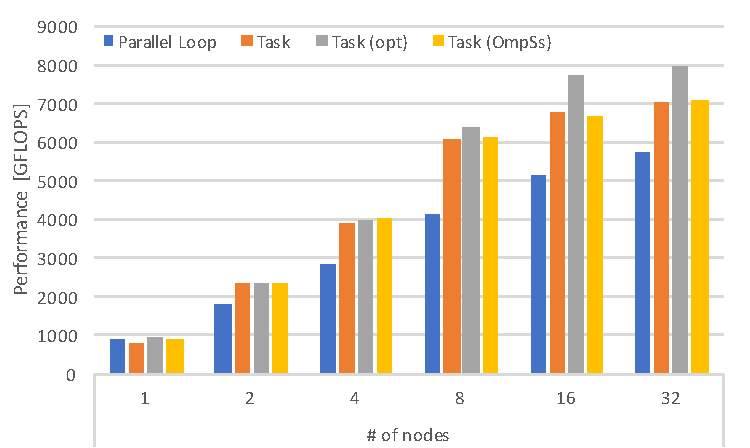
\includegraphics[bb=0 0 360 216, width=6cm]{./figure/FIG_OFP_CH3.pdf}
\hspace{1.6cm} (A) Performance
%\vspace{-3mm}
\end{center}
\end{minipage}\begin{minipage}{0.5\hsize}
\begin{center}
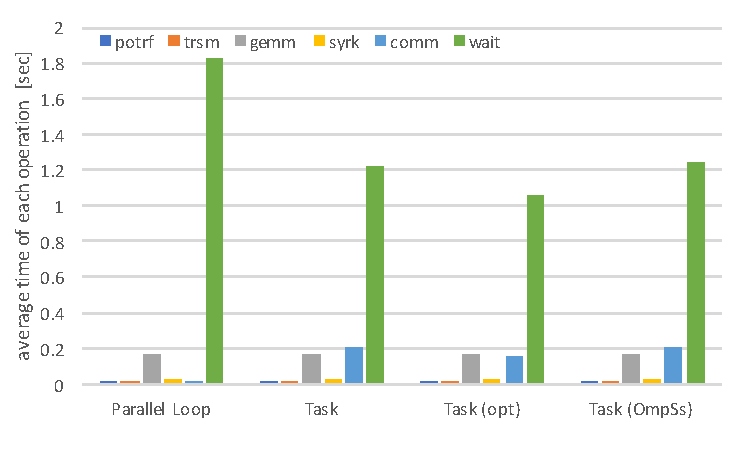
\includegraphics[bb=0 0 360 216, width=6cm]{./figure/FIG_OFP_CH_BD3.pdf}
\hspace{1.6cm} (B) Breakdown at 32 nodes execution
%\vspace{-3mm}
\end{center}
\end{minipage}
\caption{Performance and breakdown of blocked Cholesky factorization on the Oakforest-PACS system.}
\label{FIG_OFP_CH}
\end{figure*}

\begin{figure}[t]
\centering
{\scriptsize
\begin{minipage}{7.8cm}
\begin{lstlisting}
double A[nt][nt][ts*ts], B[ts*ts], C[nt][ts*ts];
#pragma xmp nodes P(*)
#pragma xmp template T(0:nt-1)
#pragma xmp distribute T(cyclic) onto P
#pragma xmp align A[*][i][*] with T(i)

#pragma xmp tasklets
for (int k = 0; k < nt; k++) {
#pragma xmp tasklet out(A[k][k]) on T(k)
    potrf(A[k][k]);

#pragma xmp tasklet gmove in(A[k][k]) out(B) on T(k:)
    B[:] = A[k][k][:];

    for (int i = k + 1; i < nt; i++) {
#pragma xmp tasklet in(B) out(A[k][i]) on T(i)
        trsm(B, A[k][i]);

#pragma xmp tasklet gmove in(A[k][i]) out(C[i]) on T(i:)
        C[i][:] = A[k][i][:];            
    }
    for (int i = k + 1; i < nt; i++) {
        for (int j = k + 1; j < i; j++) {
#pragma xmp tasklet in(A[k][i], C[j]) out(A[j][i]) on T(j)
            gemm(A[k][i], C[j], A[j][i]);
        }
#pragma xmp tasklet in(A[k][i]) out(A[i][i]) on T(i)
        syrk(A[k][i], A[i][i]);
    }
}
\end{lstlisting}
\end{minipage}
}
\caption{Blocked Cholesky factorization code in the XMP {\tt tasklet} directive}
\label{FIG_CHOLESKY}
\end{figure}

\begin{figure*}[htbp]
\begin{minipage}{0.5\hsize}
\begin{center}
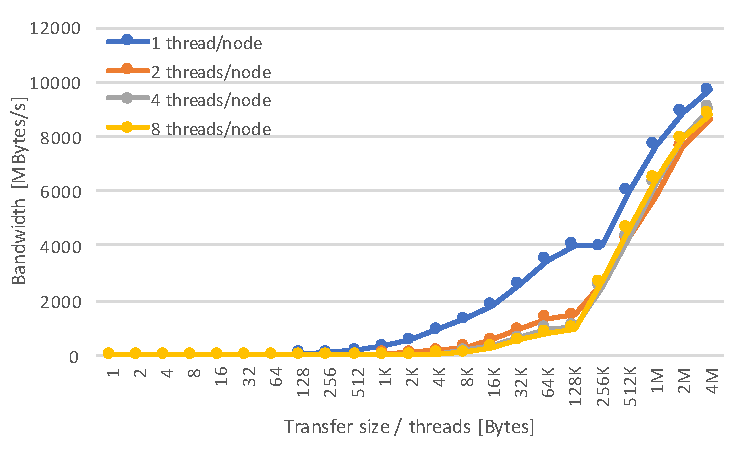
\includegraphics[bb=0 0 360 217, width=6cm]{./figure/FIG_OFP_PING_PONG.pdf}
\hspace{1.6cm} (A) Oakforest-PACS
%\vspace{-3mm}
\end{center}
\end{minipage}\begin{minipage}{0.5\hsize}
\begin{center}
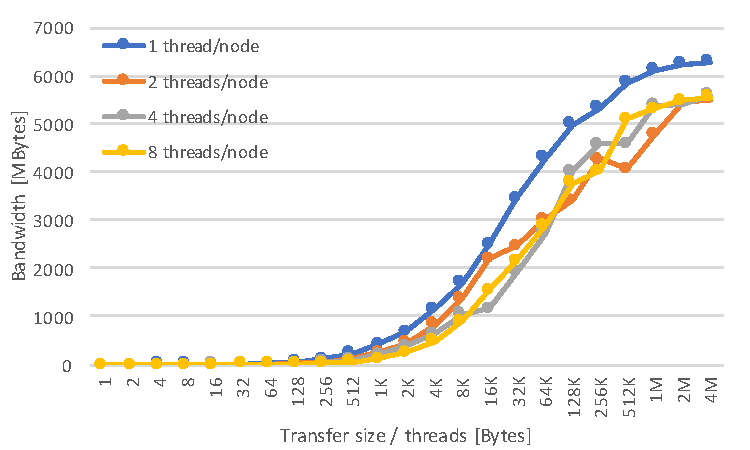
\includegraphics[bb=0 0 360 217, width=6cm]{./figure/FIG_COMA_PING_PONG.pdf}
\hspace{1.6cm} (B) COMA
%\vspace{-3mm}
\end{center}
\end{minipage}
\caption{Performance of the Ping-Pong benchmark on the Oakforest-PACS and COMA systems.}
\label{FIG_PING_PONG}
\end{figure*}

\subsection{Communication Optimization for Many-core Clusters} \label{SEC5}

In the global task parallel programming model, the communication may happen at each pair of tasks between nodes. In order to enable the communication in multithreaded environment, we may use MPI\_THREAD\_MULTIPLE as the MPI thread-safety level, because tasks executed on threads may communicate simultaneously.
We have examined the basic performance of multithreaded communications
by using the Ping-Pong benchmark. This benchmark is based on the OSU Micro-Benchmarks 5.3.2 \cite{OSU} developed by the Ohio State University.
we also show the aggregated bandwidth when multiple threads (i.e., two, four, or eight threads) communicate at the same time. Figure \ref{FIG_PING_PONG} illustrates the communication performance on the Oakforest-PACS system. The performance of multi-threaded communication with MPI\_THREAD\_MULTIPLE degrades compared to a single-threaded communication as the number of threads increases.
As with the result on the Oakforest-PACS system, the performance of communication on a single thread is better compared to that for multi-threaded communication with MPI\_THREAD\_MULTIPLE.
Therefore, the communication performance may be improved if all communications are delegated to the communication thread. To delegate the communications to a single thread, we create a global queue that is accessible by all threads, so that the tasks enqueue the communication requests into this queue and wait for the communication to complete. Meanwhile, the communication thread dequeues the requests for communication to perform the requested communications, and checks the communication completion. The communication thread executes only the communication, and the other threads perform computation tasks.

Figure \ref {FIG_OFP_CH} shows the performance and breakdown of blocked Cholesky factorization with the communication optimization denoted as ``Task (opt)''.
The ``Task (opt)'' version of blocked Cholesky factorization perform better than the multi-tasking execution with MPI\_THREAD\_MULTIPLE.
The reason for this is that the communication time decreases compared with the ``Task'' version, as shown in Figs. \ref{FIG_OFP_CH}, because of the use of the communication thread. The relative performances compared with the barrier-based ``Parallel Loop'' implementation improve to 138\% on the Oakforest-PACS systems.

\section{Retrospectives and Challenges for Future PGAS models}

Since 2007, we have been developing the XcalableMP PGAS language and its reference implementation by the Omni compiler.

In this section, the challenges for future PGAS models are presented with some retrospectives on our project.

\subsection{Low-Level Communication Layer for PGAS model}

PGAS is implemented by Remote Memory Access (RMA) providing light-weight one-sided communication and low overhead synchronization semantics.
For programmers, both PGAS and RMA are programming interfaces and offer several constructs such as remote read/write and synchronizations.

Remote Direct Memory Access (RDMA) is a mechanism (operation) to access data in remote memory by giving address in (shared) address space. 
It can be done without involving the CPU or OS at the destination node.
Recent advanced interconnect such as Cray Aries interconnect and Fujitsu Tofu of K computer and Tofu-D of Fugaku support remote DMA operations which strongly support efficient one-sided communication.

For the most PGAS runtimes, one sided communication operations such as Remote Direct Memory Access (RDMA) functions in the MPI are used to implement remote put/get operations in the PGAS languages.
Although MPI3 provides several RMA APIs as library interface,
the advantages of direct use of RMA/RDMA Operations are as follows:
\begin{itemize}
\item Multiple data transfers can be performed with a single synchronization operation.
\item Some irregular communication patterns can be more economically expressed.
\item The RDMA can be significantly faster than send/receive on systems with hardware support for remote memory access.
\end{itemize}

We found the multiple data transfers for the stencil computation can be optimized by using a single synchronization operation at the end \cite{Iwashita2018}.
As described in Chapter 3, our XMP Coarray were implemented by both MPI and Fujitsu low-level Tofu API. In case of MPI, we used “passive target” mode in MPI one-sided communication. It is noted that the MPI flush operation and synchronization do not sometimes match to implement “sync\_images”, and the complex “window” management to expose the memory as an coarray.
Finally, Fujitsu RDMA interface is much faster in K-computer.

Other problem is the communication in the multithreaded environment. As described in the previous sections, we found the performance problem of MPI\_THREAD\_MULTIPLE.
As the connection-less semantics of RDMA would be suited to communications in multithreaded environment, we believe that a new design of low-level communication layer would be a desirable solution in near future.

\subsection{XcalableMP as a DSL for stencil applications}

The Domain Specific Language (DSL) is a promising approach to make the programing easy in a specific domain. 
Many DSLs such as OpenFOAM in CFD is successful. 

Many DSLs are proposed to describe the typical stencil computation. On the other hand, we propose the mixed-language programming with XcalableMP in Chapter 5. Using this model, the main kernel of the computation can be written in XcalableMP and other controls, input/output and house-keeping operation are written by other familiar languages such as Python. In this case, a part of XMP is thought as a kind of DSL to write the stencil computation with global view programming.

 The advantages of this approach are as follows:

\begin{itemize}
\item By using the XMP global-view programming model, the stencil computation can be described in a simple loop based on its original sequential program. 
\item The stencil communication can be done by the XMP optimized stencil communication runtime. \cite{Iwashita2018}
\item The advanced optimization of the stencil operations is enabled by a set of the directives for the extended stencil optimization such as a loop unrolling and temporal blocking, added in the latest XcalableMP specification, version 1.4 \cite{XMP-Spec-1-4}.
\end{itemize}

\subsection{XcalableMP API: Compiler-free Approach}

Although many PGAS languages such as UPC and Chapel, CAF, have proposed, it is hard to say that they are full accepted by the community of parallel programming. Recently, the libraries supporting the PGAS model,
such as OpenShmem\cite{OpenShmem}, GlobalArray\cite{GlobalArray}, even MPI3 RMA, are getting popular for programming some specific applications. Furthermore, many C++ template-based design for PGAS,
such as UPC++\cite{UPC++}, DASH\cite{DASH}, are proposed as a compiler-free approach, as C++ template provides powerful abstraction mechanism. This approach may increase portability, clean separation from base compiler optimization, but a problem is that it is sometimes hard to debug in C++ template once a programmer writes wrong programs.

The approach of extending the language given by the support of the compiler, the compiler-approach, may give:
\begin{itemize}
\item A new language, or language extension provides easy-to-use and intuitive feature resulting in better productivity.
\item This approach enables the compiler analysis for further optimization, such as removal of redundant sync and selection of efficient communication.
\end{itemize}

In reality, the compiler-approach is not easy to be accepted for deployment and supports in many sites, resulting in the failure of wide dissemination.

We will have a plan to design the library interface for XcalableMP programming model, XMP API, which is aiming to provide the most equivalent programming functions by the set of libraries. 

\subsection{Global Task Parallel Programming Model for Accelerators}

The task-based programming recently supported in OpenMP 4.0 enables to expose a lot of parallelism by executing several tasks of the program in the form of task-graph. To accelerate the task-based parallel program by accelerators such as GPU and FPGA, it is useful for some tasks frequently executed in parallel to be offloaded to accelerators as an asynchronous task executed by accelerators. 

In previous section, the global task parallel programming model is presented. The next step will be that this global task parallel programming model is extended to tasks offloaded to accelerators attached to each node in accelerated clusters. 

Exploration of new high-performance architectures from programing model’s point of view is an important challenge. Future parallel architecture will be more heterogenous having many kinds of accelerators and devices attached to the nodes and directly connected between accelerators by some dedicated interconnect. To program such a complex and heterogenous parallel system, the global task parallel programming model will give a flexible and decomposable model to exploit such heterogenous high performance architecture.


\begin{thebibliography}{10}

\bibitem{FLAGSHIP2020}
  https://www.r-ccs.riken.jp/en/overview/exascalepj/
{\emph  Flagship 2020 Project (Supercomputer Fugaku)}

\bibitem{Murai2013}
Hitoshi Murai, Mitsuhisa Sato
\newblock{ An Efficient Implementation of
Stencil Communication for the XcalableMP PGAS Parallel Programming
Language,}
\newblock{\em 7th International Conference on PGAS Programming Models,}
Edinburgh, Scotland, UK (2013, Oct.).

\bibitem{Fiber}
RIKEN Advanced Institute for Computational Science (RIKEN AICS), Fiber
Miniapp Suite, fiber-miniapp.github.io (2104).

\bibitem{Murai2017} Hitoshi Murai, Masahiro Nakao, Hidetoshi Iwashita, Mitsuhisa Sato. 
\newblock {Preliminary Performance Evaluation of Coarray-based
Implementation of Fiber Miniapp Suite using XcalableMP PGAS
Language,}
\newblock{\em Second Annual PGAS Applications Workshop (PAW)}, CO, USA
(2017, Nov.).

\bibitem{CCS-QCD}
 https://www.ccs.tsukuba.ac.jp/qcd/ccsqcdsolverbenchmic/.
\emph{CCS QCD Solver benchmark program}

\bibitem{NTChem}
  https://www.r-ccs.riken.jp/software\_center/software/ntchem/overview/,
\emph{NTChem Overview}.  

\bibitem{uTofu}
FUJITSU Ltd., Development Studio uTofu User's Guide (2020, Mar.).

\bibitem{HPCAsia2018}
  Keisuke Tsugane, Jinpil Lee, Hitoshi Murai, Mitsuhisa Sato
  \newblock{ Multi-tasking Execution in PGAS Language XcalableMP and Communication Optimization on Many-core Clusters.}
  \newblock{\em HPC Asia 2018}, pp. 75-85. Tokyo, 2018.


\bibitem{OFP}
Joint Center for Advanced High Performance Computing (JCAHPC), ``Basic Specification of Oakforest-PACS'', http:{\slash}{\slash}jcahpc.jp{\slash}files{\slash}OFP-basic.pdf

\bibitem{OMPSS} D. Alejandro, A. Eduard, B. Rosa M, L. Jesus, M. Luis,
  M. Xavier, P. Judit, ``Ompss: a Proposal for Programming
  Heterogeneous Multi-Core Architectures'', Parallel Processing
  Letters, Vol.21, pp.173--193, 2011.

\bibitem{OFP}
Joint Center for Advanced High Performance Computing (JCAHPC), ``Basic Specification of Oakforest-PACS'', http:{\slash}{\slash}jcahpc.jp{\slash}files{\slash}OFP-basic.pdf

\bibitem{OSU}
``OSU Micro-Benchmarks'', http:{\slash}{\slash}mvapich.cse.ohio-state.edu{\slash}benchmarks/

\bibitem{Iwashita2018}
  Hidetoshi Iwashita, Masahiro Nakao, Hitoshi Murai, Mitsuhisa Sato.
  \newblock{``A Source-to-Source Translation of Coarray Fortran with MPI for High Performance,''}
  \newblock{\em HPC Asia 2018,} Tokyo, Japan, Jan. 2018.

\bibitem{XMP-Spec-1-4} https://xcalablemp.org/download/spec/xmp-spec-1.4.pdf,
  \emph{XcalableMP Language Specification v 1.4}.

\bibitem{OpenShmem}
http://www.openshmem.org/site/, \emph{OpenShmem}

\bibitem{GlobalArray}
https://hpc.pnl.gov/globalarrays/, \emph{Global Arrays}

\bibitem{UPC++}
  Y. Zheng, A. Kamil, M. B. Driscoll, H. Shan, K. Yelick,
  \newblock{ ``UPC++: A PGAS Extension for C++'',}
  \newblock{\em 2014 IEEE 28th International Parallel and Distributed Processing Symposium,} pp. 1105--1114, 2014.

\bibitem{DASH}
  K. Fuerlinger, T. Fuchs and R. Kowalewski,
  \newblock{ "DASH: A C++ PGAS Library for Distributed Data Structures and Parallel Algorithms,"}
  \newblock{\em 2016 IEEE 18th International Conference on High Performance Computing and Communications; IEEE 14th International Conference on Smart City; IEEE 2nd International Conference on Data Science and Systems (HPCC/SmartCity/DSS),}
  Sydney, NSW, 2016, pp. 983-990, doi: 10.1109/HPCC-SmartCity-DSS.2016.0140.

\end{thebibliography}

\end{document}


